%
% Niniejszy plik stanowi przykład formatowania pracy magisterskiej na
% Wydziale MIM UW.  Szkielet użytych poleceń można wykorzystywać do
% woli, np. formatujac wlasna prace.
%   
% Zawartosc merytoryczna stanowi oryginalnosiagniecie
% naukowosciowe Marcina Wolinskiego.  Wszelkie prawa zastrzeżone.
%
% Copyright (c) 2001 by Marcin Woliński <M.Wolinski@gust.org.pl>
% Poprawki spowodowane zmianami przepisów - Marcin Szczuka, 1.10.2004
% Poprawki spowodowane zmianami przepisow i ujednolicenie 
% - Seweryn Karłowicz, 05.05.2006
% Dodanie wielu autorów i tłumaczenia na angielski - Kuba Pochrybniak, 29.11.2016

% dodaj opcję [licencjacka] dla pracy licencjackiej
% dodaj opcję [en] dla wersji angielskiej (mogą być obie: [licencjacka,en])
\documentclass[licencjacka,en]{pracamgr}

\usepackage{graphicx} %package to manage images
\usepackage{url}
\graphicspath{ {./images/} }
\usepackage[utf8]{inputenc}
\usepackage[rightcaption]{sidecap}
\usepackage{wrapfig}
\usepackage{titlesec}

\usepackage{listings}
\usepackage{xcolor}
\usepackage{float}

\definecolor{codegreen}{rgb}{0,0.6,0}
\definecolor{codegray}{rgb}{0.5,0.5,0.5}
\definecolor{codepurple}{rgb}{0.58,0,0.82}
\definecolor{backcolour}{rgb}{0.95,0.95,0.92}

\lstdefinestyle{mystyle}{
    backgroundcolor=\color{backcolour},   
    commentstyle=\color{codegreen},
    keywordstyle=\color{magenta},
    numberstyle=\tiny\color{codegray},
    stringstyle=\color{codepurple},
    basicstyle=\ttfamily\footnotesize,
    breakatwhitespace=false,         
    breaklines=true,                 
    captionpos=b,                    
    keepspaces=true,                 
    numbers=left,                    
    numbersep=5pt,                  
    showspaces=false,                
    showstringspaces=false,
    showtabs=false,                  
    tabsize=2
}

\lstset{style=mystyle}

% Dane magistranta:
% \autor{Adam Deryło, Adrian Hess, Magdalena Pałkus, Michał Skwarek}{34234234}

% Dane magistrantów:
\autor{Adam Deryło}{432952}
\autori{Adrian Hess}{431481}
\autorii{Magdalena Pałkus}{421537}
\autoriii{Michał Skwarek}{418426}
%\autoriv{Autor nr Cztery}{432145}
%\autorv{Autor nr Pięć}{342011}

\title{Blazingly fast GPU acceleration of CCSDS Rice decoding}
\titlepl{Akceleracja GPU dekodowania CCSDS Rice}

%\tytulang{An implementation of a difference blabalizer based on the theory of $\sigma$ -- $\rho$ phetors}

%kierunek: 
% - matematyka, informacyka, ...
% - Mathematics, Computer Science, ...
\kierunek{Computer Science}

% informatyka - nie okreslamy zakresu (opcja zakomentowana)
% matematyka - zakres moze pozostac nieokreslony,
% a jesli ma byc okreslony dla pracy mgr,
% to przyjmuje jedna z wartosci:
% {metod matematycznych w finansach}
% {metod matematycznych w ubezpieczeniach}
% {matematyki stosowanej}
% {nauczania matematyki}
% Dla pracy licencjackiej mamy natomiast
% mozliwosc wpisania takiej wartosci zakresu:
% {Jednoczesnych Studiow Ekonomiczno--Matematycznych}

% \zakres{Tu wpisac, jesli trzeba, jedna z opcji podanych wyzej}

% Praca wykonana pod kierunkiem:
% (podać tytuł/stopień imię i nazwisko opiekuna
% Instytut
% ew. Wydział ew. Uczelnia (jeżeli nie MIM UW))
\opiekun{Paweł Gora\\
  Faculty of Mathematics, Informatics and Mechanics, University of Warsaw\\
  }

% miesiąc i~rok:
\date{Jun 2023}

%Podać dziedzinę wg klasyfikacji Socrates-Erasmus:
\dziedzina{ 
%11.0 Matematyka, Informatyka:\\ 
%11.1 Matematyka\\ 
% 11.2 Statystyka\\ 
11.3 Informatics, Computer Science \\ 
%11.3 Informatyka\\ 
%11.4 Sztuczna inteligencja\\ 
%11.5 Nauki aktuarialne\\
%11.9 Inne nauki matematyczne i informatyczne
}

%Klasyfikacja tematyczna wedlug AMS (matematyka) lub ACM (informatyka)
\klasyfikacja{D. Software\\
  D.1.3. Concurrent Programming\\
  I.4.2. Compression (Coding) \\ }

% Słowa kluczowe:
\keywords{CCSDS Rice coding, GPU, Compute Unified Device Architecture (CUDA)}

% Tu jest dobre miejsce na Twoje własne makra i~środowiska:
\newtheorem{defi}{Definicja}[section]

% koniec definicji

\begin{document}
\maketitle

%tu idzie streszczenie na strone poczatkowa
\begin{abstract}
\end{abstract}

\tableofcontents
%\listoffigures
%\listoftables

\chapter{Introduction}
\section{Background and motivation}
Machine learning (ML) has rapidly become a crucial tool for solving complex problems in a variety of domains, including computer vision, natural language processing, and speech recognition. However, ML pipelines can often experience significant bottlenecks due to multi-stage data processing pipelines that include loading, decoding, cropping, resizing, and other augmentations. This is particularly true when these processing steps are executed on a CPU, which is frequently the case. Since most of the machine learning training is already GPU accelerated due to ML workloads having a highly parallel nature, it is a natural progression to solve data processing bottlenecks by harnessing GPU acceleration. 

One such bottleneck is decompression of RICE-coded data, which is one of the most commonly used compression algorithms used in astronomy and astrophysics. Currently, there are only CPU-based solutions for decoding RICE-compressed data. It substantially hinders application of machine learning solutions in astronomy, especially considering the massive amount of training data already stored in RICE-compressed algorithm as well as being produced by observatories all around the world. To illustrate, just single instrument  - AIA on the Solar Dynamics Observatory (SDO) spacecraft, is producing \~67 megabits of RICE-coded data per second, of which roughly 4 TB is captured on earth \cite{sdo-data}. This amounts to a staggering 1460 TB of new data per year from not even just a single observatory, but a single measurement instrument.  

\section{Problem statement}
The problem at hand is that the current RICE decompression algorithm is computationally intensive and cannot keep up with the demand for high throughput and real-time processing. The goal of this project is to design  and develop a GPU-based RICE decompression algorithm that can significantly accelerate the decompression process and improve the speed, efficiency, and scalability of ML pipelines in astronomy applications.

\section{Research objectives}
The main objectives of this thesis are as follows:

\begin{itemize}
    \item To study the existing literature on GPU acceleration of data compression and RICE decompression.
    \item To analyze the performance of RICE decompression on a CPU and a GPU.
    \item To design and implement a GPU-accelerated RICE decompression algorithm.
    \item To evaluate the performance of the GPU-accelerated RICE decompression algorithm and compare it with the CPU-based RICE decompression algorithm.
    \item And finally, to incorporate findings into NVIDIA Data Loading Library (DALI)\cite{dali-docs}, so machine learning, as well as the astronomy community, can utilize our findings.
\end{itemize}

\section{Thesis structure}
In this thesis, we present our attempts at parallelizing the RICE decompression algorithm and CUDA-based implementations of our findings. 

 Chapter \ref{r:definitions} aims to define and explain key terms for our problem space, including the FITS file format and the RICE compression algorithm itself. In the following chapter, we review previous work on the subject. Thereafter, in chapter \ref{r:context}, the broader context of our thesis is examined. This chapter, aims to introduce the reader to the subject of GPU programming, NVIDIA's involvement in that field. Additionally, we explain core concepts of the DALI library, since it was an integral part of our project. Subsequently, in chapter \ref{r:impl} we present our solution architecture and how it ties into NVIDIA's aforementioned open-source data-loading framework called DALI. In chapter \ref{r:algo}, we propose a parallel implementation of the RICE algorithm on the GPU and describe our efforts in optimizing the parallel implementation of the RICE decoding algorithm. Chapter \ref{r:results} presents our performance and speedup results. Finally, in chapter \ref{r:conclusion}, we summarize our findings and conclude the thesis.

\chapter{Key terms}\label{r:definitions}

\section{FITS format}

\subsection{Overview of FITS}

The Flexible Image Transport System (FITS) format is an openly documented digital file format commonly utilized in the field of astronomy for storing and transferring scientific data. The International Astronomical Union FITS Working Group (IAU-FWG) \cite{fits-working-group}is responsible for developing and maintaining the FITS format, with significant influence from the worldwide astronomy community. FITS format was designed for long-term usage, providing features such as backwards compatibility and standardization \cite{fits-standard}. FITS files typically contain images, data cubes, tables of observational data, and associated metadata, including observation date, instrument name, and coordinates.

One of the key characteristics of FITS is its ability to store multiple data arrays in a single file, enabling efficient storage and transfer of large datasets. FITS files are composed of the following structures in the listed order \cite{fits-official}:
\begin{itemize}
\item Primary HDU.
\item Conforming Extensions (optional).
\item Other special records (optional, restricted).
\end{itemize}

Thus, files usually resemble the following schema \cite{fits-image}:

\begin{figure}[h]
\centering
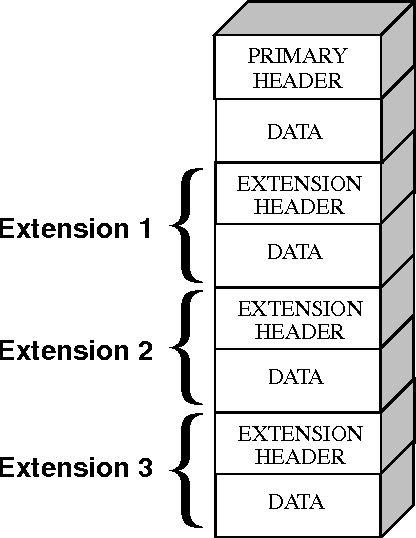
\includegraphics[scale=0.3]{fits}https://www.overleaf.com/project/637dd868a84cdd4898a13e23
\end{figure}

In every HDU including the primary one,  header contains relevant metadata as a list of key-value pairs. \cite{wikipedia} Furthermore, the most recent FITS standard published by CCSDS defines three types of standard extensions:
\begin{itemize}
\item IMAGE extensions.
\item TABLE ASCII-table extensions.
\item BINTABLE binary-table extensions.
\end{itemize}


\subsection{Compression of fits}

\subsubsection{Motivation}
In modern astronomy, observations produce huge datasets (even 12 TB per day \cite{crayondata} ) that are often archived and processed many years after their registration due to their size and quantity. Storing and managing data in compressed form is essential due to their smaller size. Compression of astronomical data is important for several reasons:
\begin{itemize}
\item Enabling storage of much more data in the same memory size.
\item Accelerating throughput between research centers.
\item Optimizing computational efficiency.
\item Following the strategy "Compress once, decompress never," many computational programs provide an interface to operate directly on FITS compressed files \cite{why-rice}. 
\item Many scientific tools are compatible and accept compressed FITS files.
\end{itemize}\\

\subsubsection{Tile compression convention}

The tiled-image compression convention refers to the method of compressing images in the FITS format using a tiling approach. In this procedure, the FITS file is divided into smaller parts called tiles. Each tile is compressed independently, enabling efficient utilization of computational resources. This approach also allows for the decoding of specific parts of the data without having to decode the entire file. The CFITSIO library implements this convention and supports the following data compression algorithms: Rice, Hcompress, PLIO, and GZIP \cite{rice-comp}. Among these algorithms, the Rice algorithm is very efficient \cite{fpack} for compressing FITS files due to its higher speed and compression ratio compared to the others mentioned \cite{rice-comp}.

\subsubsection{Review of employed compression algorithms}

The most commonly used algorithms employing the tile compression convention are as follows \cite{rice-comp}:

\begin{itemize}
\item Rice: A simple and efficient lossless algorithm mentioned above.
\item Hcompress: A compression algorithm that uses wavelet transform followed by quantization and quadtree coding. By omitting the quantization step, Hcompress can also function as a lossless data compression algorithm.
\item PLIO (Piecewise Linear Image Compression with Optimization): An image compression algorithm that approximates an image using straight line segments.
\end{itemize}

\subsection{Benchmarks of various algorithms and why RICE was chosen}
The Rice compression algorithm is faster than alternatives like GZIP in terms of compression time for astronomical data (about 2-3 times faster) and results in a higher compression ratio of the input file by about 1.4 times \cite{rice-comp}. According to some papers, the Rice algorithm can also be faster in decompression \cite{why-rice}. These results indicate that using tile compression algorithms like Rice is more efficient for compressing astronomical data.

\section{CCSDS RICE coding}

\subsection{Golomb coding}
\subsubsection{History}
Golomb coding is losless data compression method named after its inventor, Solomon W. Golomb. It was first introduced in 1966. \cite{golomb-original}
\subsubsection{How it works}
In simple words, Golomb coding is a technique that is particularly effective for encoding non-negative integers. It uses a combination of unary and binary encoding to achieve efficient compression. In this procedure, index values $i$ are divided into equal groups of size $m$. \cite{golomb-coding-work} Next, the codeword are constructed from a unary code, that describe each group, followed by constant-size code $v_i$, that indicates the remainder of the index, that has been encoded.  Then, Golomb code residual is generated according to following formula \cite{golomb-coding-work}:
$$v_i = i - \left\lfloor\frac{i}{m}\right\rfloor \cdot m$$
\subsubsection{Pseudo Code}

\subsubsection{Example}

\subsection{Rice coding}
\subsubsection{History, how it is different from Golomb coding}
In RICE coding, invented by Robert F. Rice, that is subset of Golomb coding, using special $m$ values, according to formula: $m = 2^k$ \cite{golomb-coding-work}. This allows for the use of simple arithmetic bit-shifting operations that work in constant time, thereby accelerating the compression process.

The RICE algorithm is lossless, bit-wise data compression algorithm that uses a set of variable-length codes to compress data. As a lossless data compression algorithm \cite{rice-basics}, RICE is able to retrieve the full data from its compressed form without losing any part of the original data. The bit-wise algorithm operates on single bits (in contrast to byte-wise, which operates on single bytes), enabling greater compression due to the smaller granularity of the data they work with.

The essence of this algorithm is to use these codes to change symbols that are expected to be more frequent into shorter code words. The algorithm works on independently encoded data blocks, eliminating the need to transfer information between different packets. This improves performance and makes the RICE algorithm performance independent of data packet size \cite{rice-codes}.


\subsubsection{Pseudo Code}
Example of RICE encoding pseudo code is shown on following figure \cite{golomb-wikipedia}: \\
\begin{figure}[h]
\centering
\includegraphics[scale=0.5]{Rice_pseudocode}
\end{figure}

\subsubsection{Example}

\subsection{CCSDS RICE}
\subsubsection{How it differs from general implementation}
CCSDS RICE is a compression algorithm developed by the Consultative Committee for Space Data Systems (CCSDS) for space data applications. It is designed to achieve efficient compression while allowing reversible decompression, meaning the original data can be completely reconstructed from the compressed representation. CCSDS RICE uses a context selection mechanism to adaptively choose the optimal coding scheme for different data contexts.

CCSDS RICE operates by dividing the input data into blocks and encoding each block separately. It uses a combination of Golomb-Rice coding and Huffman coding techniques to encode the data efficiently. The Golomb-Rice coding is employed to handle the larger magnitude values, while Huffman coding is used for smaller magnitude values. The context selection mechanism helps determine which coding scheme is applied to each block based on the characteristics of the data.

For example, image encoding using the CCSDS RICE algorithm involves dividing the image into blocks of pixels and applying a predictive coding technique to compute and encode differences between the predicted value and the actual value. A variant of the Golomb coding is used, which uses a fixed-length prefix of binary zeros followed by a unary code to represent the quotient and remainder of the difference value \cite{rice-codes}. Unlike Golomb coding, where the number of bits needed to write the remainder depends on a variable parameter, the RICE algorithm uses data blocks of a constant size, resulting in a constant number of needed bits that is always a power of two. The prefix size typically depends on the characteristics of the image being compressed.

\subsubsection{Algorithm walk through}



The RICE algorithm consists of two main parts: a preprocessor and an adaptive entropy coder \cite{rice-basics}:
\begin{itemize}
\item The preprocessor is responsible for data processing before the actual compression. This part of the algorithm converts the input data into preprocessed samples and passes them to the Adaptive Entropy Coder.
\item The Adaptive Entropy Coder assigns shorter codes to symbols that occur more frequently and longer codes to symbols that occur less frequently. This part of the algorithm converts the preprocessed samples into the final encoded bit sequence.
\end{itemize}

\hfill \break
\hfill \break
\hfill \break
\hfill \break
This process can be ilustrated into following figure \cite{rice-basics}:
\hfill \break
\hfill \break
\centerline{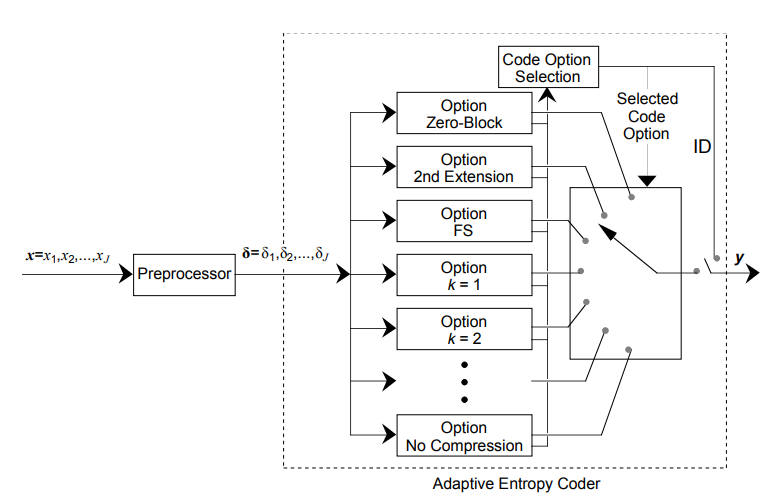
\includegraphics[scale=1.05]{RICE_encoder_architecture}}


% TODO:\\
% 1.Why compress at all? \\ 
% 2.Tile compression convention.\\
% 3.Review of employed compression algorithms. (and why rice is the best) \\ 

% Soruces: 
% https://heasarc.gsfc.nasa.gov/fitsio/fpack/O1.5.pdf  (1) 
% https://arxiv.org/pdf/0903.2140.pdf
% (2,3) 

\chapter{Related work\label{r:related}}

\section{Overview of the problem space}
The acceleration of the Golomb-Rice algorithm has garnered some attention in the literature, with most of the work focusing on the compression side of the problem. In particular, researchers have extensively studied Golomb parameter selection due to its critical role in determining achieved compression ratios. However, regarding throughput acceleration, the majority of the research has focused on implementing FPGA-based hardware acceleration for both compression and decompression. Notably, some software (CPU-based) approaches have been implemented, leveraging input format to achieve decoding throughput improvements from 1 Gbps to 4 Gbps \cite{fpga-dec}.

As for GPU-based acceleration, Xianyun Wu et al. evaluated the feasibility of GPU acceleration for the coding side of the issue in their study “Is the CCSDS Rice Coding Suitable for GPU Massively Parallel Implementation?” \cite{gpu-rice}. The authors achieved a six-fold speed up over the single-threaded CPU counterpart and concluded that CCSDS Rice coding contains numerous flow control instructions, significantly affecting the instruction throughput. These findings highlight the potential benefits of GPU-based acceleration for the coding side of the problem, but also suggest that further work is necessary to optimise CCSDS Rice coding for efficient GPU-based implementations.

\section{Current RICE decoding solutions in context of FITS}
To the best of our knowledge, the industry standard for compression and decompression of CCSDS Rice coded FITS files is achieved through the use of two standalone programs, fpack and funpack \cite{funpack-man}. These programs offer a unique advantage as they directly read and write the compressed FITS image format, eliminating the need for creating an uncompressed version of the file [why-rice](https://www.notion.so/why-rice-ab9d5ef4bfbd474bb049b8d3b0e047c2) . Additionally, fpack and funpack rely on the aforementioned tile compression convention and support multiple compression algorithms, including Hcompress, GZIP, and IRAF, apart from RICE \cite{funpack-user}. Both programs are included with CFITSIO\cite{funpack-man} , a FITS File Subroutine Library that is maintained by NASA’s High-Energy Astrophysics Science Archive Research Center (HEASARC) \cite{cfitsio}.

Regarding machine learning and data science workflows, where python is a prevailing programming language \cite{dev-survey}, either astropy or fitsio packages are mainly utilised \cite{astropy} \cite{fitsio} . While fitsio package is simply a Python wrapper for CFITSIO, astropy builds upon the PyFits package and is thus is a purely Pythonic implementation of various FITS File subroutines. Nevertheless, when it comes to compression, astropy accesses CFITSIO to support the FITS Tile Compression convention \cite{astropy}, what in the end makes them equivalent in terms of throughput in most cases. On that note, fitsio is shown to outperform astropy on the data sets consisting mainly of small files ($\sim0.3$ MB) \cite{astropy vs fitsio}, and thus it will be used for various Python-based benchmarks.

In summary, the fitsio and astropy packages offer convenient interfaces for accessing FITS files and decompressing CCSDS Rice encoded data in Python-based workflows. However, it should be noted that all of these packages rely on the same CPU-based RICE decompression algorithm implemented by funpack. While this algorithm has proven to be effective in achieving high compression ratios for a wide range of data types, it is limited in terms of its processing speed and throughput due to its CPU-based nature. As such, there is a growing interest in exploring alternative solutions that leverage emerging hardware technologies such as GPUs and FPGAs to accelerate the RICE decompression process. Such solutions have the potential to significantly improve the performance and efficiency of CCSDS Rice encoding and decoding in various domains, including machine learning, data science, and space science.

\chapter{Broader context}\label{r:context}

\section{NVIDIA}
NVIDIA Corporation is a technology company known for designing and manufacturing graphics processing units (GPUs). Its professional line of GPUs are used in workstations for applications in such fields as architecture, engineering and construction, media and entertainment, automotive, scientific research, and manufacturing design. 

In addition to designing hardware, NVIDIA has made significant efforts to develop software tools and libraries that facilitate the use of their GPUs in scientific computing. Among these efforts, CUDA stands out as one of the most notable contributions. CUDA, which stands for Compute Unified Device Architecture, is a parallel computing platform and programming model that enables researchers to harness the power of GPUs for scientific computing tasks \cite{cuda-about}. With CUDA, developers can write programs in C, C++, and Fortran that can take advantage of the parallelism of GPUs to accelerate computations \cite{cuda-toolkit-official}. This has led to significant performance improvements for many scientific computing applications, including those in the fields of astrophysics, computational biology, and machine learning. 

To further support the use of GPUs in scientific computing, NVIDIA provides a range of software libraries that are optimised for use with CUDA. These include cuBLAS, cuFFT, and cuSPARSE, which provide high-performance implementations of common linear algebra, signal processing, and sparse matrix operations that are essential for many scientific computing applications\cite{nvidia-math-libs}. By offering these libraries, NVIDIA has made it easier for researchers and developers to take advantage of the power of GPUs in scientific computing.

\section{CUDA}
% hsitory and background 

% core concepts
% kernels

% stream based concurrency model


%%\begin{itemize}
%\item {https://www.nvidia.com/en-us/about-nvidia/}
%\item {https://research.nvidia.com/publication/2021-12_evolution-graphics-processing-unit-gpu}
%\item https://www.nvidia.com/en-us/technologies/
%\item https://www.nvidia.com/en-us/data-center/ampere-architecture/
%\item https://developer.nvidia.com/cuda-zone
%\end{itemize}

\section{NVIDIA DALI}

The NVIDIA Data Loading Library (DALI) is a high-performance, portable, and open-source library for data loading and pre-processing in deep learning applications. It provides a collection of highly optimised building blocks for loading and processing image, video, and audio data. DALI can be used as a drop-in replacement for built-in data loaders and data iterators in popular deep learning frameworks, such as TensorFlow, PyTorch, and MXNet \cite{dali-docs}. \\
\\

\centerline{\includegraphics[scale=0.3]{images/dali.png}}

DALI addresses the problem of the CPU bottleneck by offloading data pre processing to the GPU. To do so DALI relies on its own execution engine, built to maximise the throughput of the input pipeline. This results in significant performance improvements for deep learning applications that require complex, multi-stage data processing pipelines \cite{blogpost}. 


\subsection{Core concepts}
In DALI, the central component is the data processing pipeline, which consists of a symbolic graph connecting data nodes through operators. These operators receive inputs, perform various data processing operations, and generate outputs. DALI categorises its operators into three types based on their backend: CPU, Mixed, and GPU. The CPU operators handle data on the CPU, while Mixed operators transfer data from the CPU to the GPU for processing, and GPU operators handle data entirely on the GPU. The pipeline itself is defined in Python in an imperative manner similarly to how object definition is implemented in other deep learning frameworks, such as Pytorch or Tensorflow. Nonetheless, after instantiation pipeline is actually executed under the hood by the code written in C++ which allows for more efficient asynchronous processing. \cite{blogpost}   Here is an example of pipeline definition: \\ 

\begin{lstlisting}[language=Python]
from nvidia.dali import pipeline_def, fn

@pipeline_def  
def my_pipeline():
    img_files, labels = fn.readers.file(file_root="image_dir", seed=1)
    mask_files, _ = fn.readers.file(file_root="mask_dir", seed=1)
    images = fn.decoders.image(img_files, device="mixed")
    masks  = fn.decoders.image(mask_files, device="mixed")
    return images, masks, labels

pipe = my_pipeline(batch_size=4, num_threads=2, device_id=0)
pipe.build()
\end{lstlisting}

Which  results in following data processing graph: \cite{dali-docs} \\

\centerline{\includegraphics[scale=0.5]{images/dali-flow.png}}

Among many other optimizations, such architecture allows for data prefetching, that is, preparing batches of data ahead of time before they are requested. This ensures that the framework always has data readily available for the next iteration. The purpose of data prefetching is twofold: firstly, it helps to mask the latency associated with preprocessing, which becomes particularly crucial when the processing time varies significantly across iterations. Secondly, it mitigates the bottleneck caused by input/output (IO) operations. \cite{blogpost}

\subsection{Reader operators}

While in general, all operators have input and output there a three notable exceptions. Those are  readers, random number generators and external\_source operators and can be treated as a data sources for the whole processing graph\cite{blogpost}. In fact, at the hearth of architecture of our proposed solution for solving RICE decoding induced bottlenecks is the introduction of new type of a reader operator able of handling RICE coded FITS files. Anyways, lets glance through the abstract logic of the Reader Operators. All readers consist of data loading and reading components.

The data loading component (Loader) encapsulates logic of loading data into a buffer allocated either in host (CPU) or device (GPU) memory. Implementations of Loaders differ depending on the file format type nonetheless generally their either simply copy data or use memmap to speed up the process if possible \cite{dali-readers}.
The reader component (Reader) is responsible for orchestrating whole data reading ordeal. Broadly, speaking on initialization it starts prefetching thread that employs previously mentioned loaders to preemptively fill batch buffer. Further in this setup up faze, reader allocates the output buffer according to user passed arguments or automatically deducing from the first fetched sample.  Also it is often here when various checks on the loaded data are being run for example verifying that all samples contain images, audio of conforming dimensions and or type.  However, this part of logic is naturally often overwritten by the deriving implementations of readers for various data formats \cite{dali-readers}.  

Without getting into the wheat of specific implementations we can discern one more phase of data reading which every reader operator must implement, that is RunImpl. In this method, reader operator fills the output buffer with data so next operators in processing pipeline can access it. Further, on this stage many reader operators execute data manipulations such as decoding to unify output and allow for greater level of abstraction in use of subsequent operators \cite{dali-readers}. 

\chapter{Project stages and solution architecture}\label{r:impl}

\section{Project stages}
Our work on the project began with a comprehensive literature review focused on identifying potential solutions to mitigate the RICE decompression bottleneck. The review also aimed to gain an understanding of the current implementations of RICE decompression, including the industry standard CFITSIO. The primary objective of this initial stage was to acquire a strong conceptual foundation to inform the subsequent phases of the project.

Following the literature review, the project moved onto the implementation phase, which began with the development of a CPU-based FITS reader operator and incorporating it into DALI. This version of the FITS reader operator relied on CFITSIO and was designed as a base solution to branch of and  benchmark against in subsequent phases of the project. 

After the development of the CPU-based FITS reader operator, we concurrently worked on a CUDA kernel that would accelerate RICE decompression as well as a necessary infrastructure to incorporate it into DALI. On this stage, we iterated multiple times trying out various approaches which will be described in later chapters.

Furthermore, on this stage we have started working on synthetic benchmarks of our solution. Their synthetic nature stem from the fact that we tested just the raw speed of reading generated files without testing impact of the rest of data loading pipeline. This allowed us to make more educated choices when iterating through various approaches without spending much effort on building up more holistic bench marking suite and at the cost of not knowing how various speed techniques employed in data reading stages of the data processing graph impact total throughput. More on that in the chapter on benchmarking. 

Finally, we evaluated the performance of the GPU-accelerated RICE decompression algorithm using a range of synthetic and real-world benchmarks. These benchmarks were designed to test the speed, efficiency, and scalability of the algorithm across a range of data sizes and processing loads. More on that in the dedicated chapter on benchmarks. 

Overall, the implementation phase of the project involved the development of a comprehensive solution architecture that addressed the problem of RICE decompression bottlenecks in ML pipelines in astronomy applications. The architecture consisted of a parallelized CUDA-based RICE decompression kernel, a new RICE compressed FITS reader operator, and a range of performance benchmarks.

In the subsequent section we will go through a architecture of the final solution which was incorporated into DALI.

\section{Architecture and implementation details}
In order to incorporate our findings into the DALI library we had to create a new reader operator that would handle FITS files and in the end also allow for acceleration of their decompression by parallizing on GPUs. Here is a UML diagram of both versions of FITS readers:\\

\centerline{\includegraphics[scale=0.5]{images/fits_reader_uml.png}}

In following sections we will go though each newly introduced component documenting its implementation details.
\subsection{FitsReader}
The FitsReader class is a base class that is responsible for reading and loading FITS (Flexible Image Transport System) files in a DALI data pipeline. It is implemented as a template class, taking the Backend and Target types as template parameters. The class inherits from the DataReader class, which is a base class for all data reader operators and contains less context depended methods such as GetSample(), which retrieves a specific sample from the already prefetched batch. In the FitsReader class we have implemented two core functionalities - data reading setup in SetupImpl() method, and api interface definition. 

The SetupImpl() method takes a vector of OutputDesc objects and a Workspace as parameters. The function first calls the SetupImpl() function of the base class to start prefetching data and wait for a consumable batch. Then, it determines the number of outputs and samples, and resizes output\_desc, a container from which any subsequent operator will get data, accordingly. 
Finally, it validates the dimensions and data types of each sample in the batch, ensuring consistency among samples. 

Declaration of api interface was done using preexisting DALI\_SCHEMA macro which allows for registering a visible form python interface of the newly created operator. Additionally it auto generates documentation for that operator which you can find here \cite{fitsreader-docs}.

%% describe implementation of API interface

\subsection{FitsReaderCPU}
The FitsReaderCPU class is a derived class of FitsReader specifically designed for the CPU backend. The constructor of FitsReaderCPU takes an OpSpec object as a parameter and calls the constructor of the base class. It also initializes the loader\_ member variable by calling the InitLoader() function with the FitsLoaderCPU type and other par\_descameters obtained from the OpSpec in order to pass along user specified parameters. Furthermore, it overrides the RunImpl() function to provide the implementation for reading FITS files on the CPU. 


\subsection{FitsReaderGPU}
The main purpose of the FitsReaderGPU component is to efficiently read and decompress FITS files on a GPU, taking advantage of the parallel processing capabilities of modern GPUs. This allows for faster data loading and processing, which is especially beneficial when dealing with large datasets or real-time applications.

The implementation utilizes CUDA, a parallel computing platform and programming model, to perform the decompression of the FITS data on the GPU. It includes a kernel function called "rice\_decompress" that performs our CCSDS RICE decompression algorithm, in case to be read files require decompression. The kernel function is templated to support different data types, such as uint8\_t, uint16\_t, and uint32\_t, ect. corresponding to the pixel data types commonly found in FITS files. Thus, if else logic is being handled by 
the RunImpl() method which is executed by the CPU. By doing so we aimed at reducing on device branch prediction and offloading it to better suited for that task CPU. 

During execution, the FitsReaderGPU component reads the compressed data from the FITS file and applies the Rice decompression algorithm in parallel on the GPU. The decompressed data is then optionally rescaled using the provided scaling factors (bscale and bzero) and stored in the output tensors. If the FITS file is not compressed, the data is directly copied from host memory to the output tensors allocated on the device memory.

\subsection{FitsLoader}

The FitsLoader component is responsible for implementing logic of loading FITS files from host memory into a struct consisting of meta data and a container of Tensor objects on which the FitsReader operator operates. It is implemented as a template class, taking the Backend and Target types as template parameters. The FitsLoader class inherits from the FileLoader class, which is a base class for all file loader operators in the pipeline. It overrides the PrepareEmpty() and ReadSample() methods to handle the preparation and reading of FITS files.

During construction, the FitsLoader class takes the OpSpec object and a boolean flag indicating whether to shuffle the files after each epoch. OpSpec contains parameters such as number of outputs, which are mapped to the number of HDUs which should be read from each file.  Given that information FitsLoader infers what HDU indices are ought to be read. 

The PrepareEmpty() method sets the target object to an empty state, preparing it to hold the loaded data. The ReadSample() method reads a sample from the FITS file, processing each extension specified by the HDU indices argument retrieved from the OpSpec object.

In the ReadSample() method, the FITS file is opened, and the number of HDUs (Header Data Units) in the file is determined. The target object is resized to accommodate the specified number of HDUs. For each extension specified by the HDU indices, the method moves to the corresponding HDU, reads the header, and stores it in the target object. It then resizes and resets the specific output in the target object based on the shape and data type specified in the header. After resizing the output, the method calls the ReadDataFromHDU() method, which is a virtual function that needs to be implemented in derived classes. This function reads the actual data from the HDU and populates the target object accordingly. Finally, the method sets the metadata and file path in the target object and moves to the next sample or wraps around to the beginning of the shard if necessary.

\subsection{FitsLoaderCPU}

The FitsLoaderCPU class is a derived class of FitsLoader specifically designed to work with FitsReaderCPU. In essence it provides the implementation for the aforementioned ReadDataFromHDU() helper function ReadDataFromHDU(). As our main focus was to provide GPU acceleration 
of the decoding process of FITS files we entirely resorted to using 
CFITSIO function calls to parse, read and decode files if necessary in the CPU version of this operator.  

\subsection{FitsLoaderGPU}
The FitsLoaderGPU is a  GPU counterpart of the previously examined class. Similarly, it also
derived from the base FitsLoader class and provides implementation of ReadDataFromHDU() method. Despite the GPU suffix in the name it actually doesn't load the contentment's of 
the provided files into the GPU memory but rather simply copies it to the host memory. 
The distinguishing logic encapsulated in this component is that in case the loaded file 
is compressed it extracts its raw compressed data, and groups it into the tiles so the decompression kernel in the FitsReaderGPU can concurrently process each tile. More on 
behavior of the kernel will be in the next chapter. 

\subsection{Utils}

While we primarily relied on the functions provided by the CFITSIO library to parse the contents of FITS files, we encountered certain limitations that required us to implement additional functionalities ourselves.

One such example was the need to extract raw data from compressed files without the requirement of decompressing them first. As CFITSIO did not offer a straightforward way to access the raw data of compressed files, we developed a custom function to handle this specific task. This implementation allowed us to efficiently access the necessary data for further processing without unnecessary decompression steps.

Moreover, we introduced several other utilities to augment the capabilities of our solution. We created handlers for file streams, enabling smooth interaction with file I/O operations. Additionally, we developed classes to map the metadata contained in the headers of each read HDU (Header Data Unit) into objects that could be conveniently used throughout the codebase. All in all, these utility additions created more seamless experience of working with FITS files inside the DALI library.

\subsection{Testing and CI/CD} 
To enhance the development speed and ensure the functionality of our new features in the DALI library, we adopted two types of tests: end-to-end tests and unit tests.

End-to-end tests were introduced first chronologically, as they allowed us to verify the correct behavior of our solution and determine if we could proceed with implementing new features and optimizations. For these tests, we utilized NumPy and Random python packages to generate arrays of pixel values with various dimensions for all supported data types. Using astropy, we saved the generated data in FITS format to establish a ground truth for the tests. Subsequently, we compared the data read by the Fits-Reader on both back-ends to the pre-generated ground truth, ensuring their consistency. We utilized the nose2 testing framework to facilitate these tests.

In addition to the black-box testing approach, we also developed unit tests for the more algorithmically complex components. They
were welcomed addition during our development cycles since with the introduction of certain performance optimizations such as loop unrolling, parts of our code base tended to become less readable. For example, one such component that necessitated unit testing was the aforementioned raw data extraction utility. 

Apart from running tests locally, they were also included into the CI/CD pipeline, so no pull request would be merged into the NVIDIA DALI repository if introduced changes broke our tests. 
% if time allows write more about CI\CD pipepline 

\chapter{GPU acceleration of RICE decoding}

\section{Naive approach}\label{r:algo}

During CCSDS Rice compression, the image is divided into a grid of rectangular tiles (Internal Tiled-Image Compression). Each tile of pixels is individually compressed and then stored in rows of a variable length array column in a FITS binary table. Tiles are by default row-wise, but in fact they can be of any size.

The above considerations immediately lead to the idea that each tile should also be decompressed individually. While extracting the compressed data, we also calculate the start and end indexes of all tiles and pass this information to the GPU kernel. Then we can simply launch as many threads as possible and delegate each of them to handle the decompression of a single tile. In the default case of row-wise tiles, all rows in the image are decoded simultaneously.

\section{Optimizing asynchronous data transfer}
% CUDA has it, and what it allows
Compute Unified Device Architecture (CUDA) since its very beginnings supports asynchronous data transfer between host and device and vice versa. This feature allows for non blocking execution with respect to the host code as well as well as enables possibility of overlapping kernel execution and data transfers. 
% How it works??? this section depends on CUDA
% section in Context, don't know if we should explain whole concurency model
Asynchronous data transfer ties deeply into the CUDA concurrency model. As such when data is copied from host memory to the device for the processing, one has to specify a stream with which the copy operation will be synchronized. Thus, we place H2D copy of the compressed data and subsequent kernel execution on the same stream allowing for host to move on to
processing other files, and in turn initiating more kernel executions in the same span of time. The effects of such optimizations
can be illustrated by the following diagram: 

\centerline{\includegraphics[scale=0.3]{images/async/cuda1.png}}

In our case, we are not too bothered about device to host (D2H) data transfers since subsequent operators are expected to
work on compatible memory. I.e. if the reader operator back-end is set to GPU then it reads data into the GPU memory and
following data augmentations can also rely on GPU acceleration. In the end, deep learning network that will be the final recipient of the data is also expected to work with device memory. This eliminates completely potential bottlenecks caused by the back and forth 
data transfers on a PCIe data bus with its limited bandwidth. More on that in the ensuing section.   



\section{Minimizing data transfers}
When being careless with the structure of the data and the manner in which it is copied over to the device memory we might become stifled in our pursuit of performance by the time spend on doing I/O operations instead of performing any meaningful computation. 

This problem is of such importance due to the vast discrepancy between bandwidth between device (GPU) and its memory (651.3 GB/s in case of NVIDIA TITAN V graphics card \cite{titan-v})  and the peak bandwidth between host memory and device memory (32 GB/s on PCIe x16 Gen4 \cite{pcie}). This discrepancy holds up even in case of proprietary solutions such as NV-Link \cite{gpu-interconnect}, making a transfer of data between host and device a natural bottleneck \cite{gpu-bottelnecks}.
Nonetheless, there are several principles that help to combat lose of performance due to this 
predicament. And all of those techniques have one common aim - that is utilizing the H2D bandwidth to the fullest. 

% recheck the data about single burst vs payload size 
Firstly, we resorted to aggregating numerous small transfers into a single larger transfer
of continuous memory. Why such optimization might be helpful? 
Single payload sent using PCIe or NV-link interconnect has anywhere from 128B to 512B \cite{pcie}.
Thus when we copy non contiguously allocated memory part of the bus is unutilized as it transmits irrelevant data. 
As for why doing a lot of memcpy calls is not beneficial might seem quite intuitive but
the reason is twofold. First, we might overwhelm driver that has handle those
calls. Secondly, we are naturally under utilizing the bandwidth of the interconnect. This effect saturates
at certain point (around $2^{22} B$) where larger chunks of data do not improve the bandwidth \cite{gpu-interconnect}. Nonetheless,
improvement till that point is of an exponential nature.
To harness those improvements before initializing H2D transfer we ensure that the to be transferred data representing RICE coded images is allocated in a contiguous manner even if that means that it has to be re-copied in the host memory.  


Secondly, we experimented with the utilization of page-locked (or "pinned") memory. Normally,
data allocations on the host (CPU) are pageable. However, direct access to data from pageable host memory is not possible on the GPU. Therefore, when a data transfer is initiated from pageable host memory to device memory, the CUDA driver necessitates the allocation of a temporary page-locked, or "pinned," host array. This process involves copying the host data to the pinned array and subsequently transferring the data from the pinned array to the device memory \cite{pinned_memory}. The following diagram illustrates this sequence of operations:
\centerline{\includegraphics[scale=0.3]{images/memory/pinned.png}}\\
Basically, when using pinned memory we can avoid unnecessary copy operations. This has been shown to reduce the execution times 
of various algorithms but the order of 2. However, the improvements weren't consistent accords all benchmarks, especially in 
cases where the workloads were more GPU bound than CPU bound \cite{pinned_comparison}.  


\\

%% how this helps



Lastly, as already mentioned in the asynchronous data transfer section, overlapping data transfers between the host and the device with kernel execution and other data transfers can lead to improved overall system efficiency. This overlap allows for concurrent execution of these operations, minimizing idle time and maximizing resource utilization.




\section{Kernel 3.0}


\chapter{Results and Analysis}\label{r:results}
This chapter presents the benchmark results of our project. The benchmark tests are used to measure the performance of our project, particularly in terms of how the incorporation of DALI affects the performance of processes handling large data sets. 

Additionally, these tests act as a form of validation. We developed our project in collaboration with NVIDIA and the Solar Dynamics Observatory (SDO). These benchmarks provide an opportunity to confirm that our system operates as expected, ensuring that the work we've done meets our anticipated outcomes.

Importantly, benchmarks also help us establish a reproducible testing environment. This ensures that our findings are not an artifact of a specific set of conditions, but rather results that can be replicated under similar parameters. In the context of this study, it is worth noting that the same dataset was used across both stages (section \ref{dataset}). This consistency in data usage further enhances the comparability and reliability of our results.

Performance benchmarking was divided into two stages:
\begin{itemize}
    \item Synthetic Benchmarks: comparing the speed of DALI's readers. FITS decoding on CPU versus GPU (section \ref{benchmark}).
    \item Application Benchmarks: measuring the speedup of the learning process of a U-Net-based CHeSS deep learning model \cite{CHeSS} with DALI integration (section \ref{chess}).
\end{itemize}

This double testing process allows us to fully evaluate our system's performance. On one hand, Synthetic Benchmarks let us measure the speed of individual operations. That's really useful, because it lets us figure out which parts of our system are slower and might need some work. On the other hand, Application Benchmarks help us see how these speeds affect the learning process of our model in a real-world scenario. We believe that this comprehensive approach to benchmarking will give us valuable insights into the overall performance and areas of improvement of our project.

\section{Experimental Setup}

The computational experiments for this study were conducted on a dedicated machine equipped with a high-performance CPU and GPU to facilitate the extensive data handling and processing tasks.

The primary graphics processing unit (GPU) used for the experiments was an NVIDIA GV100 [TITAN V] graphics card \cite{titan}. This GPU is part of NVIDIA's Volta architecture line and is renowned for its high computational power and proficiency in handling data-intensive tasks. The GV100 [TITAN V] supports a 64-bit memory interface and operates at a clock speed of 33MHz, providing a substantial computational resource for deep learning applications.

The central processing unit (CPU) used in this work was an Intel(R) Core(TM) i9-10920X CPU \cite{intel}, which operates at a base frequency of 3.50GHz, with a maximum frequency of up to 4.80GHz. This high-performance CPU features 12 cores and 24 threads.


\section{\label{dataset}Dataset Description}

We used the dataset from the Solar Dynamics Observatory's (SDO) 193 Angstrom telescope, capturing solar activity throughout 2011. It contains 1349 FITS files, each an image of the sun (Figure \ref{fits_photo}).

Of particular interest within these images are "coronal holes," areas where the solar magnetic field reaches out into space instead of looping back onto the sun's surface. Studying these areas is crucial for solar physicists because they can generate solar wind streams, which influence space weather conditions on Earth \cite{coronal-holes}.


\begin{figure}[h]
    \vspace{1cm} 
    \centering
    \begin{minipage}{.45\textwidth}
        \centering
        \includegraphics[width=\textwidth]{sdo1.png}
    \end{minipage}\hfill
    \begin{minipage}{.45\textwidth}
        \centering
        \includegraphics[width=\textwidth]{sdo2.png}
    \end{minipage}
    \caption{Examples of photos from SDO 193 Angstrom telescope \cite{sdo-photos}}
    \label{fits_photo}
\end{figure}

We use this dataset for two primary purposes in our project. For synthetic benchmarks, the large size of the dataset allows us to measure speed and efficiency of our computational tools and methods under heavy data loads. For the application benchmarks, we use this dataset to train the CHeSS model \cite{CHeSS} in different configurations, with and without use of DALI. By presenting the model with this dataset, it learns to detect and segment coronal holes. Training the model with this data on various configurations allows us to see how different settings influence its performance.

\section{\label{benchmark}Synthetic benchmarks}
\subsection{Overview of Tests}
This test evaluates the performance of the GPU-accelerated RICE decompression algorithm and compares it to the CPU-based RICE decompression algorithm. Moreover, the results were also compared with those from using Python's astropy and fitsio. The script was designed to test only the speed of FITS file reading. The impact of the rest of the data loading pipeline was deliberately excluded.

The dataset used for the tests was the one mentioned previously \cite{sdo}, consisting of 1349 FITS files. Considering the large size and complexity of these files, the experiment provided a realistic scenario for testing and comparing the performance of both types of hardware.

A batch size of 32 with 24 threads was selected as it resulted in the best test outcomes. Applying these values across all tests ensured consistency in the results and guaranteed that any observed differences in performance could be attributed to the hardware, not changes in processing parameters.



\subsection{Metrics}
To effectively evaluate the performance of our proposed solution for the DALI FITS file reader, we adopted several key metrics:
\begin{itemize}
    \item \textbf{Throughput}: Defined as the number of FITS files processed per unit of time (specifically, per second). Higher throughput corresponds to more efficient data handling and faster processing times, which are particularly critical for large datasets.
    \item \textbf{Latency}: Represents the time duration required to process a single FITS file, from initiation to completion. Lower latency indicates a faster response and swift data processing, contributing to overall system efficiency.
    \item Furthermore, we took into consideration the \textbf{mean time}, \textbf{total time}, and \textbf{variance} in our performance measurements. These statistics offer a more detailed view of our solution's performance.
\end{itemize}


\subsection{Results}
The results are presented in table \ref{CPUvsGPU} and in figure \ref{CPUvsGPUjpeg}.
The results showed a pronounced difference in performance of our solution between the two environments. The GPU outperformed the CPU by a significant margin, achieving a throughput of 48.8 files/s compared to the CPU's 4.47 files/s. The GPU also boasted a substantially lower latency at 0.0205 s, a stark contrast to the CPU's 0.224 s. These numbers clearly highlight the advantage of utilizing GPU resources when working with substantial and complex datasets like the ones used in this project.

% - results of FItsReaderCPU ( === cfitiso) vs FitsReaderGPU
% - restuls against python packages astropy & fitsio

\renewcommand{\arraystretch}{2}
\begin{table}[H]
    \centering
    \begin{tabular}{|c|c|c|c|c|}
        \hline
        & FitsReaderCPU & FitsReaderGPU & Astropy & FITSIO \\\hline
        Throughput (files/\textit{s}) & 4.47 & 48.80 & x & x \\\hline
        Latency (\textit{s}) & 0.22 & 0.02 & x & x \\\hline
        Total time (\textit{s}) & 301.61 & 27.64 & x & x \\\hline
        Mean time per batch (\textit{s}) & 7.01 & 0.64 & x & x \\\hline
        Variance (\textit{s}) & 6.41 & 0.07 & x & x \\\hline
    \end{tabular}
    \caption{\label{CPUvsGPU} Results of synthetic benchmarks.}
\end{table}

%TODO: zorbic przewy z gory i z dolu obrazkow by bylo czytelne
\begin{figure}[htbp]
    \centering
    \vspace{1cm} % Dodaj poziomą przestrzeń tutaj
    \begin{minipage}{.45\textwidth}
        \centering
        \includegraphics[width=\textwidth]{throughput.png}
        \subcaption{Throughput}
    \end{minipage}\hfill
    \begin{minipage}{.45\textwidth}
        \centering
        \includegraphics[width=\textwidth]{latency.png}
        \subcaption{Latency}
    \end{minipage}

    \vspace{1cm} % Dodaj poziomą przestrzeń tutaj
    
    \begin{minipage}{.45\textwidth}
        \centering
        \includegraphics[width=\textwidth]{mean_time.png}
        \subcaption{Mean time}
    \end{minipage}\hfill
    \begin{minipage}{.45\textwidth}
        \centering
        \includegraphics[width=\textwidth]{total_time.png}
        \subcaption{Total time}
    \end{minipage}
    \caption{Results of synthetic benchmarks.}
    \label{CPUvsGPUjpeg}
\end{figure}



\section{\label{chess}Application Benchmarks}

Application benchmarks serve as end-to-end evaluations of how our solution performs in real-world applications. A main aspect of this assessment involves implementing various data preprocessing pipelines in the CHeSS project. By utilizing different technologies for this purpose, we can carry out a comparative analysis of their performance. Integrating NVIDIA's DALI into the CHeSS model introduces improvements to the model's data handling capabilities, offering a possibility of speeding up the computations. The inclusion of our custom FITS file handling function in DALI and its subsequent use in the CHeSS model demonstrates a practical approach to improving performance.

\subsection{CHeSS Overview}
The Coronal Hole Semantic Segmentation (CHeSS) project \cite{CHeSS} is an initiative focused on the application of deep learning for the detection and segmentation of solar coronal holes. These coronal holes, characterized by lower temperatures and densities compared to surrounding regions, are key to understanding solar winds and the Sun’s magnetic field dynamics.

CHeSS capitalizes on the power of deep learning, utilizing a U-Net-based architecture, a form of convolutional neural network (CNN) acclaimed for its high performance in tasks such as biomedical image segmentation. The U-Net architecture is particularly adept at preserving spatial hierarchies, making it well-suited to the problem of semantic segmentation.

In terms of input data, CHeSS operates on a dataset of solar images, which are subsequently processed and analyzed to identify and delineate the coronal holes. To facilitate this process, the project makes use of the FITS file format. 


\subsection{DALI Integration in CHeSS}

The integration of DALI into the CHeSS codebase replaced the TensorFlow Dataset API with DALI's readers.FITS and readers.Numpy for handling FITS and .npy files respectively, and applying operations like resizing. We introduced command-line flags --use\_dali and --GPU to the CHeSS code, enabling optional utilization of DALI and the selection between CPU and GPU for data handling. Integration performance was evaluated by comparing the results of two configurations:
\begin{itemize}
\item Original Implementation: This replicates the training methodology used by the original authors of the CHeSS project, employing the fitsio library and TensorFlow with data preprocessing handled on the CPU and model training executed on the GPU. This scenario serves as the baseline for subsequent comparisons.
\item DALI-Accelerated GPU Implementation: In this configuration, we introduced our DALI-enhanced functionality for FITS file handling and moved both data preprocessing and model training to the GPU. This setup allows us to assess the impact of our DALI integration in a GPU-oriented context, specifically using our accelerated decompression algorithm.
\end{itemize}

In both configurations, we adopted the following hyperparameters: a batch size of 4, which provided satisfactory results, and 10 epochs, aligning with the original approach. This ensured a consistent testing environment across both setups.

The primary metric for this performance comparison was execution time, rather than training results. We were particularly interested in comparing the runtimes of the CHeSS code with and without the --use\_dali flag. This comparison was intended to show the effectiveness of DALI integration in terms of performance and speed of operations, providing insight into the potential benefits of DALI for similar projects.

\subsection{Results}

The results from the GPU tests demonstrated DALI's proficiency in reducing execution times. The execution time of CHeSS code with DALI for a batch size of 4 was found to be 482.97 s, what was approximately 142.6 seconds faster than without DALI on the GPU, a substantial difference considering the nature of tasks performed. This performance enhancement was not limited to GPU tests (figure \ref{CHeSS}). 

Preliminary results from the CPU tests also showed an approximated 30\% performance enhancement with the integration of DALI (table \ref{CHeSS}).



% 


\renewcommand{\arraystretch}{2}
\begin{table}[H]
    \centering
    \begin{tabular}{|c|c|c|}
        \hline
        & Original & DALI accelerated (GPU) \\\hline
        Time (\textit{s}) & 658 & 483  \\\hline
    \end{tabular}
    \caption{\label{CHeSS} Performance of CHeSS code with and without DALI (Batch size 4)}
\end{table}

\begin{figure}[ht]
\centering
\includegraphics[width=\textwidth]{nvidia-template.png}
\caption{\label{application-results}Results of Application Benchmarks}
\end{figure}


Overall, the benchmarking phase provided compelling evidence for the effectiveness of DALI's integration into the CHeSS code, and the performance enhancements realized from this integration underline DALI's potential benefits for similar projects in the future.


\section{Analysis of results}

This section provides an analysis and summary of the results obtained from our experimental evaluation, where we compared the performance of data processing with DALI integrated into the processing pipeline. 

In our synthetic benchmark tests, we observed a notable performance difference between using the CPU and the GPU. The GPU outperformed the CPU by a significant margin, achieving a much higher throughput (files processed per second) and much lower latency (time taken to process each file). This highlights the benefits of using GPU-accelerated processing when dealing with large and complex datasets.

In the application benchmark tests, we compared the performance of the CHeSS model when trained with the original data handling pipeline and with our DALI-enhanced pipeline. We found that the integration of DALI into CHeSS is a strategic move to leverage the power of modern GPUs, optimize data handling, and ultimately expedite the training process. 


In light of these results, the incorporation of DALI into deep learning pipelines, as illustrated with the CHeSS code, can be seen as a crucial tool for researchers dealing with vast and complex astronomical datasets. As we continue to generate and gather more extensive solar datasets, tools like DALI will be useful in handling the computational challenges that arise. 

\chapter{Conclusion}\label{r:conclusion}

\section{Summary of findings}
\section{Contributions}
\section{Future work}


\chapter{Authors’ Contributions}
Authors’ contributions to the project were as following: 


\begin{itemize}
    \item Adam Deryło 
    \begin{itemize}
        \item Initial implementation of FITS Reader CPU
        \item Initial implementation of FITS Reader GPU
        \item Performance improvements of solution via asynchronous data transfer
    \end{itemize}

    \item Adrian Hess
    \begin{itemize}
        \item Research on FITS standards and conventions
        \item Research on RICE compression algorithm 
    \end{itemize}

    \item Magdalena Pałkus 
    \begin{itemize}
        \item  Initial implementation of FITS 
        Reader CPU
        \item  Implementation and execution of Synthetic Benchmarks 
        \item Implementation and execution of Application Benchmarks 
    \end{itemize}    

    \item Michał Skwarek 
    \begin{itemize}
        \item  Research of current solutions
        \item Research on possible parallization of decoding process
        \item Work on CUDA kernel
        
    \end{itemize}   
\end{itemize}




\begin{thebibliography}{99}
	\addcontentsline{toc}{chapter}{Bibliography}

        \bibitem{rice-basics} {Rice lossless algorithm},
        \url{https://www.irjet.net/archives/V3/i2/IRJET-V3I2267.pdf} 4.05.2023

        \bibitem{sdo-data} {The Atmospheric Imaging Assembly (AIA) on the Solar Dynamics Observatory (SDO)},
        \url{https://link.springer.com/article/10.1007/s11207-011-9776-8} 8.06.2023


        \bibitem{fits-official} {FITS documentation},
        \url{https://fits.gsfc.nasa.gov/fits_documentation.html} 4.05.2023

        \bibitem{fpga-dec} {A High Throughput No-Stall Golomb-Rice Hardware Decoder},
        \url{https://ieeexplore.ieee.org/document/6545997} 4.05.2023 

        \bibitem{rice-codes} {Rice codes},
        \url{https://experiencestack.co/rice-codes-cdee6f63a546} 4.05.2023

        \bibitem{fits-image} {Fits schema},
        \url{https://www.semanticscholar.org/paper/IN-TR-O-2-2-.-2-FITS-File-Format/e87b988b4413122d0b610889e4f85da6e33cae21} 4.05.2023
        
        \bibitem{gpu-rice} {Is the CCSDS rice coding suitable for GPU massively parallel implementation?},
        \url{https://www.spiedigitallibrary.org/conference-proceedings-of-spie/8183/1/Is-the-CCSDS-rice-coding-suitable-for-GPU-massively-parallel/10.1117/12.896893.short?SSO=1} 4.05.2023 
        
        \bibitem{why-rice} {Astronomical Tiled Image Compression: How \& Why},Skwarek
        \url{https://heasarc.gsfc.nasa.gov/fitsio/fpack/O1.5.pdf} 4.05.2023 
        
        \bibitem{rice-comp} {Lossless Astronomical Image Compression and the Effects of Noise},
        \url{https://arxiv.org/pdf/0903.2140.pdf} 4.05.2023 

        \bibitem{funpack-man} {Funpack home page},
        \url{https://heasarc.gsfc.nasa.gov/fitsio/fpack/} 4.05.2023 

        \bibitem{funpack-user} {Fpack and Funpack User's Guide},
        \url{} 4.05.2023 

        \bibitem{cfitsio} {CFITSIO home page},
        \url{https://heasarc.gsfc.nasa.gov/fitsio/} 4.05.2023

        \bibitem{dev-survey} {The State of Developer Ecosystem 2022 by JetBrains},
        \url{https://www.jetbrains.com/lp/devecosystem-2022/} 4.05.2023

        \bibitem{fitsio} {Fitsio python package},
        \url{https://pypi.org/project/fitsio/} 4.05.2023

        \bibitem{astropy} {Astropy python package},
        \url{https://pypi.org/project/astropy/} 4.05.2023

        \bibitem{nvidia-math-libs} {Accelerating GPU Applications with NVIDIA Math Libraries},
        \url{https://developer.nvidia.com/blog/accelerating-gpu-applications-with-nvidia-math-libraries/} 4.05.2023

        \bibitem{cuda-refresh} {The CUDA Programming Model},
        \url{https://developer.nvidia.com/blog/cuda-refresher-cuda-programming-model/} 4.05.2023

        \bibitem{cuda-about} {About CUDA},
        \url{https://developer.nvidia.com/about-cuda} 4.05.2023

        \bibitem{open-source} {DALI SLA},
        \url{https://docs.nvidia.com/deeplearning/dali/sla/index.html} 4.05.2023

        \bibitem{dali-docs} {DALI Documentation},
        \url{https://docs.nvidia.com/deeplearning/dali/user-guide/docs/index.html} 4.05.2023

        \bibitem{blogpost} {Rapid Data Pre-Processing with NVIDIA DALI},
        \url{https://developer.nvidia.com/blog/rapid-data-pre-processing-with-nvidia-dali/} 4.05.2023

        \bibitem{dali-graph} {DALI Data Processing Graph},
        \url{https://docs.nvidia.com/deeplearning/dali/user-guide/docs/pipeline.html#data-processing-graphs} 4.05.2023 

        \bibitem{dali-readers} {DALI reader operators source code},
        \url{https://github.com/NVIDIA/DALI/tree/main/dali/operators/reader} 4.05.2023

        \bibitem{cuda-toolkit-official} {CUDA toolkit},
        \url{https://developer.nvidia.com/cuda-toolkit} 4.05.2023

        \bibitem{async-mem-blog} {CUDA toolkit},
        \url{https://developer.nvidia.com/blog/how-overlap-data-transfers-cuda-cc/} 9.06.2023

        \bibitem{cuda-wikipedia} {CUDA toolkit},
        \url{https://en.wikipedia.org/wiki/CUDA#Programming_abilities} 9.06.2023
        

        \bibitem{fits-working-group} {FITS Working Group},
        \url{https://fits.gsfc.nasa.gov/iaufwg/} 4.05.2023

        \bibitem{golomb-original} {Golomb original},
        \url{http://urchin.earth.li/~twic/Golombs_Original_Paper/} 4.05.2023

        \bibitem{golomb-coding-work} {Golomb coding},
        \url{https://www.sciencedirect.com/topics/engineering/golomb-code} 4.05.2023

        \bibitem{golomb-wikipedia} {Golomb wikipedia},
        \url{https://en.wikipedia.org/wiki/Golomb_coding} 4.05.2023

        
        \bibitem{fitsreader-docs} {Documentation for the FitsReader operator},
        \url{https://docs.nvidia.com/deeplearning/dali/user-guide/docs/operations/nvidia.dali.fn.experimental.readers.fits.html#nvidia.dali.fn.experimental.readers.fits} 8.06.2023
        

        \bibitem{fits-standard} {FITS stanard},
        \url{https://fits.gsfc.nasa.gov/standard40/fits_standard40aa-le.pdf} 4.05.2023

        \bibitem{wikipedia} {wikipedia},
        \url{https://en.wikipedia.org/wiki/FITS} 4.05.2023

        \bibitem{crayondata} {crayondata},
        \url{https://www.crayondata.com/how-does-nasa-use-big-data/} 4.05.2023

        \bibitem{fpack} {fpack},
        \url{https://heasarc.gsfc.nasa.gov/fitsio/fpack/} 4.05.2023
        
        \bibitem{funpack} {Fpack and Funpack User's Guide},
        \url{https://heasarc.gsfc.nasa.gov/FTP/software/fitsio/c/docs/fpackguide.pdf} 4.05.2023 
        \bibitem{astropy vs fitsio} {Astropy \& Fitsio speed comparison},
        \url{https://gist.github.com/ysBach/10bf843233e821dbc5fc50e2a3d2dc8f} 4.05.2023 
        
        \bibitem{dali} DALI,
        \url{https://developer.nvidia.com/dali} 4.05.2023

        \bibitem{pinned_memory} How to optimize data transfers in CUDA,
        \url{https://developer.nvidia.com/blog/how-optimize-data-transfers-cuda-cc/} 9.06.2023

        \bibitem{titan-v} TITAN V specification,
        \url{https://www.techpowerup.com/gpu-specs/titan-v.c3051} 9.06.2023    

        
        
        % graphs that show how how big writes boost bandwith; although this saturates at 2^16B
        % also info about NVLink and other data transfer solutions and their perf; 
        \bibitem{gpu-interconnect} Evaluating Modern GPU Interconnect,
        \url{https://ieeexplore.ieee.org/stamp/stamp.jsp?tp=&arnumber=8763922} 9.06.2023

        % source for info data data transfers are the major problem
        \bibitem{gpu-bottelnecks} Graph processing on GPUs: Where are the bottlenecks?,
        \url{https://ieeexplore.ieee.org/abstract/document/6983053} 10.09.2023

        \bibitem{pcie}  Understanding PCIe performance for end host networking
        \url{https://dl.acm.org/doi/abs/10.1145/3230543.3230560}, 10.09.2023

        \bibitem{pinned_comparison} Comparing unified, pinned, and host/device memory allocations for memory-intensive workloads on Tegra SoC \url{https://onlinelibrary.wiley.com/doi/epdf/10.1002/cpe.6018} 12.09.2023

        \bibitem{sdo} {SDO AIA Coronal Hole dataset},
        \url{https://rattie.orc.gmu.edu/nextcloud/index.php/s/NpoiranMBaBSgj5}

        \bibitem{CHeSS}{CHeSS: Coronal Hole Semantic Segmentation},
        \url{https://github.com/raphael-attie/CHeSS}

        \bibitem{coronal-holes}{Description of coronal holes.},
        \url{https://www.swpc.noaa.gov/phenomena/coronal-holes}
        
        \bibitem{titan}{Description of GPU used for testing}
        \url{https://www.nvidia.com/en-us/titan/titan-v/}

        \bibitem{intel}{Description of CPU used for testing}
        \url{https://www.intel.pl/content/www/pl/pl/products/sku/198012/intel-core-i910920x-xseries-processor-19-25m-cache-3-50-ghz/specifications.html}

        \bibitem{sdo-photos}{The Active Sun from SDO: 193 Angstroms}
        \url{https://svs.gsfc.nasa.gov/3981}
        % DALI section: 
        
        

        
        
\end{thebibliography}

\end{document}


%%% Local Variables:
%%% mode: latex
%%% TeX-master: t
%%% coding: latin-2
%%% End:
